\documentclass{article}
\usepackage{fancyhdr}
\usepackage{ctex}
\usepackage{listings}
\usepackage{graphicx}
\usepackage[a4paper, body={18cm,22cm}]{geometry}
\usepackage{amsmath,amssymb,amstext,wasysym,enumerate,graphicx}
\usepackage{float,abstract,booktabs,indentfirst,amsmath}
\usepackage{array}
\usepackage{booktabs}
\usepackage{multirow}
\usepackage{url}
\usepackage{diagbox}
\renewcommand\arraystretch{1.4}
\usepackage{indentfirst}
\setlength{\parindent}{2em}
\usepackage{enumitem}
\setmonofont{DejaVu Sans Mono}
\usepackage{listings}
\usepackage{xcolor}
\usepackage{makecell}
\setCJKmonofont{黑体}
\usepackage{tikz}
\usepackage{tabularx}
\usetikzlibrary{positioning, arrows.meta}
\lstset{
    % language = C,
    xleftmargin = 3em,xrightmargin = 3em, aboveskip = 1em,
	backgroundcolor = \color{white}, % 背景色
	basicstyle = \small\ttfamily, % 基本样式 + 小号字体
	rulesepcolor= \color{gray}, % 代码块边框颜色
	breaklines = true, % 代码过长则换行
	numbers = left, % 行号在左侧显示
	numberstyle = \small, % 行号字体
    numbersep = -14pt, 
    keywordstyle=\color{purple}\bfseries, % 关键字颜色
    commentstyle =\color{red!50!green!50!blue!60}, % 注释颜色
    stringstyle = \color{red}, % 字符串颜色
    morekeywords={ASSERT, int64_t, uint32_t},
	frame = shadowbox, % 用(带影子效果)方框框住代码块
	showspaces = false, % 不显示空格
	columns = fixed, % 字间距固定
} 
\lstset{
    sensitive=true,
    moreemph={ASSERT, NULL}, emphstyle=\color{red}\bfseries,
    moreemph=[2]{int64_t, uint32_t, tid_t, uint8_t, int16_t, uint16_t, int32_t, size_t}, emphstyle=[2]\color{purple}\bfseries,
    }
%--------------------页眉--------------------%
\pagestyle{fancy}
\fancyhead[L]{华东师范大学}
\fancyhead[R]{East China Normal University}
\fancyhead[C]{}
\fancyfoot[C]{-\thepage-}
\renewcommand{\headrulewidth}{1.5pt}
%--------------------标题--------------------%
\begin{document}
\begin{center}
  \LARGE{{\textbf{\heiti 华东师范大学软件工程学院实验报告}}}
  \begin{table}[H]
    \centering
    \begin{tabular}{p{2cm}p{4cm}<{\centering}p{1cm}p{2cm}p{4cm}<{\centering}}
      实验课程:    & 计算机网络 & \quad & 年\qquad 级: & 2023级      \\ \cline{2-2} \cline{5-5}
      实验编号:    & Lab 05     & \quad & 实验名称:    & UDP
      \\ \cline{2-2} \cline{5-5}
      姓\qquad 名: & 王海生     & \quad & 学\qquad 号: & 10235101559 \\ \cline{2-2} \cline{5-5}
    \end{tabular}
  \end{table}
\end{center}
\rule{\textwidth}{1pt}

\tableofcontents

%--------------------正文--------------------%
\section{实验目的}
\begin{enumerate}[noitemsep, label={{\arabic*})}]
  \item 学会通过Wireshark获取UDP消息
  \item 掌握UDP数据包结构
  \item 掌握UDP数据包各字段的含义
  \item 了解UDP协议适用领域
\end{enumerate}
\section{实验内容与实验步骤}
\subsection{实验内容}

\subsubsection{获取 \texttt{UDP} 消息}

启动 \texttt{Wireshark},在菜单栏的捕获 \(\to \)选项中进行设置,选择已连接的以太网,设置捕获过滤器为 \texttt{udp} ,将混杂模式设为关闭。

点击开始,打开浏览器,在地址栏中输入网址浏览,例如 \texttt{www.baidu.com}
或者在命令行中输入 \texttt{nslookup www.baidu.com} 查询DNS服务器
如果没有DNS解析,在命令行中输入 \texttt{ipconfig /flushdns} 清空 \texttt{DNS} 缓存
( \texttt{ipconfig /displaydns}在 \texttt{windows} 下可以使用来获取当前的 \texttt{DNS}缓存)

然后停止捕获。

\subsubsection{分析 \texttt{UDP} 包}
选择一个数据帧,分析其\texttt{UDP}包头字段。


通过查看UDP消息的详细信息,回答以下问题:
\begin{enumerate}[label={\arabic*})]
  \item \texttt{UDP}数据报头中的\texttt{Length}字段包括哪些部分?\texttt{UDP}有效载荷,还是\texttt{UDP}有效载荷加上\texttt{UDP}头的总长度?还是\texttt{UDP}有效载荷和\texttt{UDP}头以及低层协议的头部三者总长度?
  \item \texttt{UDP}校验和为多少位?
  \item 整个\texttt{UDP}头部的长度是多少字节?
\end{enumerate}

启动命令行,输入\texttt{ipconfig}获得计算机的\texttt{IP}地址,与数据包中的\texttt{Source Port}比较。

为了了解UDP在实践中是如何进行传输的,观察数据包的IP头部并思考以下问题:
\begin{enumerate}[label={\arabic*})]
  \item 将上层协议标识为\texttt{UDP}的\texttt{IP}头部的协议字段值为多少?

  \item 查看源\texttt{IP}地址与目的\texttt{IP}地址都不是你的计算机的\texttt{IP}地址的数据包,并给出这些数据包的目的\texttt{IP}地址。

  \item 一般\texttt{UDP}消息的长度是多少?
\end{enumerate}



\subsubsection{问题讨论}


\begin{enumerate}[noitemsep]
  \item 了解基于\texttt{UDP}的应用程序的流量,查看数据包大小和丢失率。

  \item 探索流和实时应用程序,查看哪些使用\texttt{UDP}以及哪些使用\texttt{TCP}进行传输。

\end{enumerate}



\subsection{实验步骤}

\begin{enumerate}[noitemsep, label={{\arabic*})}]
  \item 启动\texttt{Wireshark},在菜单栏的捕获\(\to \)选项中进行设置,选择已连接的以太网,设置捕获过滤器为\texttt{udp},将混杂模式设为关闭,然后开始捕获。
  \item 在命令行中输入 \texttt{nslookup www.baidu.com} 查询 \texttt{DNS}服务器

        \begin{lstlisting}
    PS> nslookup www.baidu.com
  \end{lstlisting}
  \item 打开 \texttt{Wireshark},停止捕获。
  \item 分析捕获到的\texttt{UDP}数据包,并回答相关问题。
  \item 问题讨论
\end{enumerate}

\section{实验环境}


\begin{itemize}[noitemsep]
  \item 操作系统:\texttt{Windows 11 家庭中文版 23H2 22631.2715}
  \item 网络适配器:\texttt{Killer(R) Wi-Fi 6 AX1650i 160MHz Wireless Network Adapter(201NGW)}
  \item \texttt{Wireshark}:\texttt{Version 4.2.0 (v4.2.0-0-g54eedfc63953)}
  \item \texttt{wget}:\texttt{GNU Wget 1.21.4 built on mingw32}
\end{itemize}


\section{实验结果与分析}

\subsection{获取 \texttt{UDP} 消息}

打开 \texttt{Wireshark},在菜单栏的捕获 \(\to \)选项中进行设置,选择已连接的以太网,设置捕获过滤器为 \texttt{udp},将混杂模式设为关闭。

\begin{figure}[H]
  \centering
  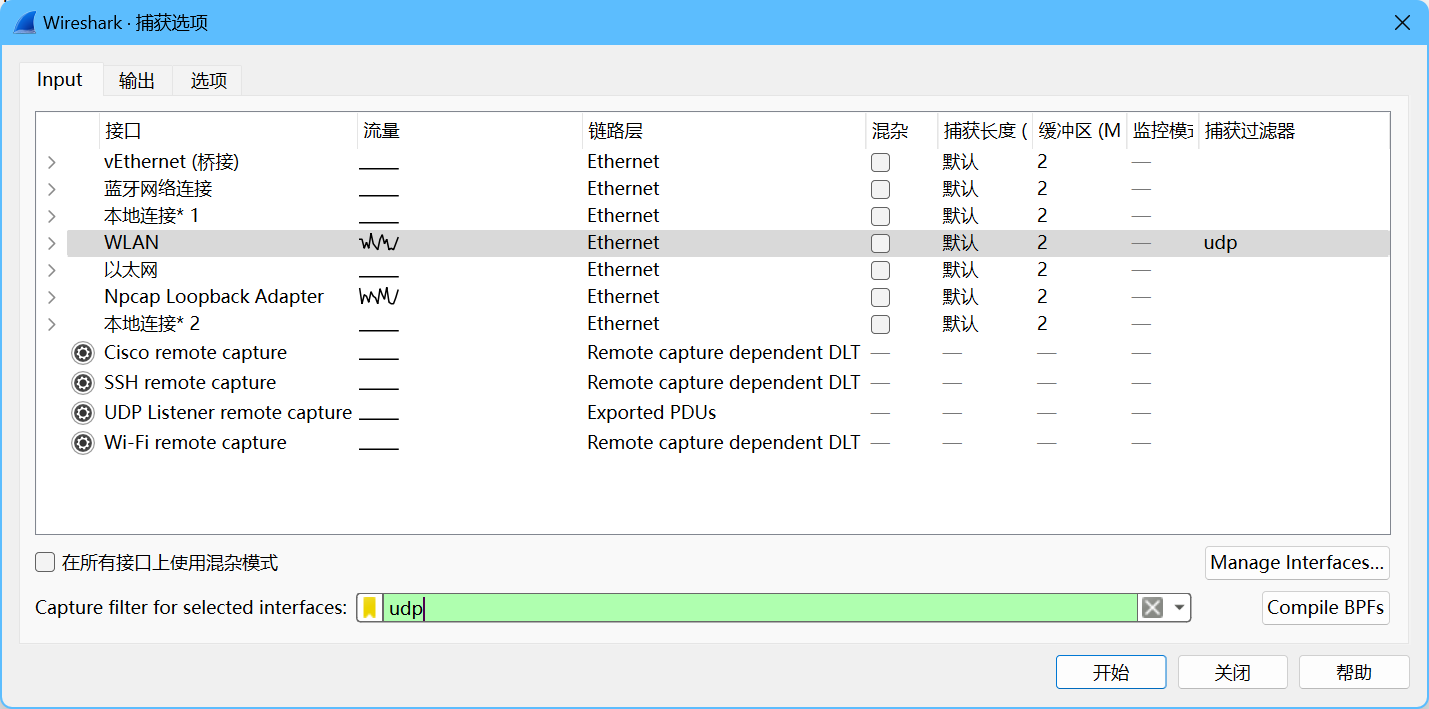
\includegraphics[width=0.8\textwidth]{img/1.png}
  \caption{设置捕获过滤器}
\end{figure}

点击开始,在命令行中输入 \texttt{nslookup www.baidu.com} 查询 \texttt{DNS}服务器。

\begin{figure}[H]
  \centering
  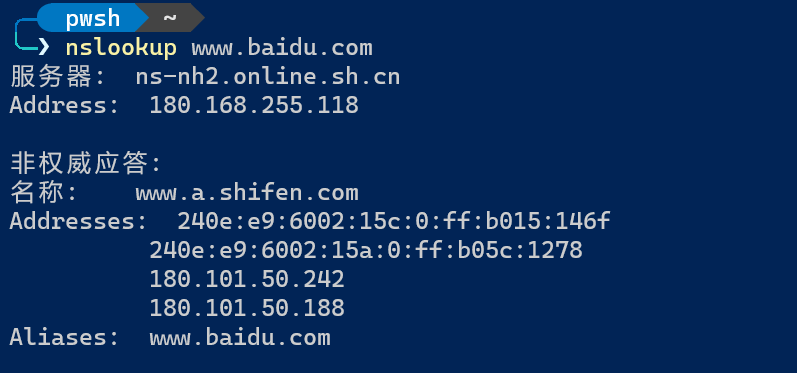
\includegraphics[width=0.8\textwidth]{img/2.png}
  \caption{查询 \texttt{DNS} 服务器}
\end{figure}

捕获结果如下:

\begin{figure}[H]
  \centering
  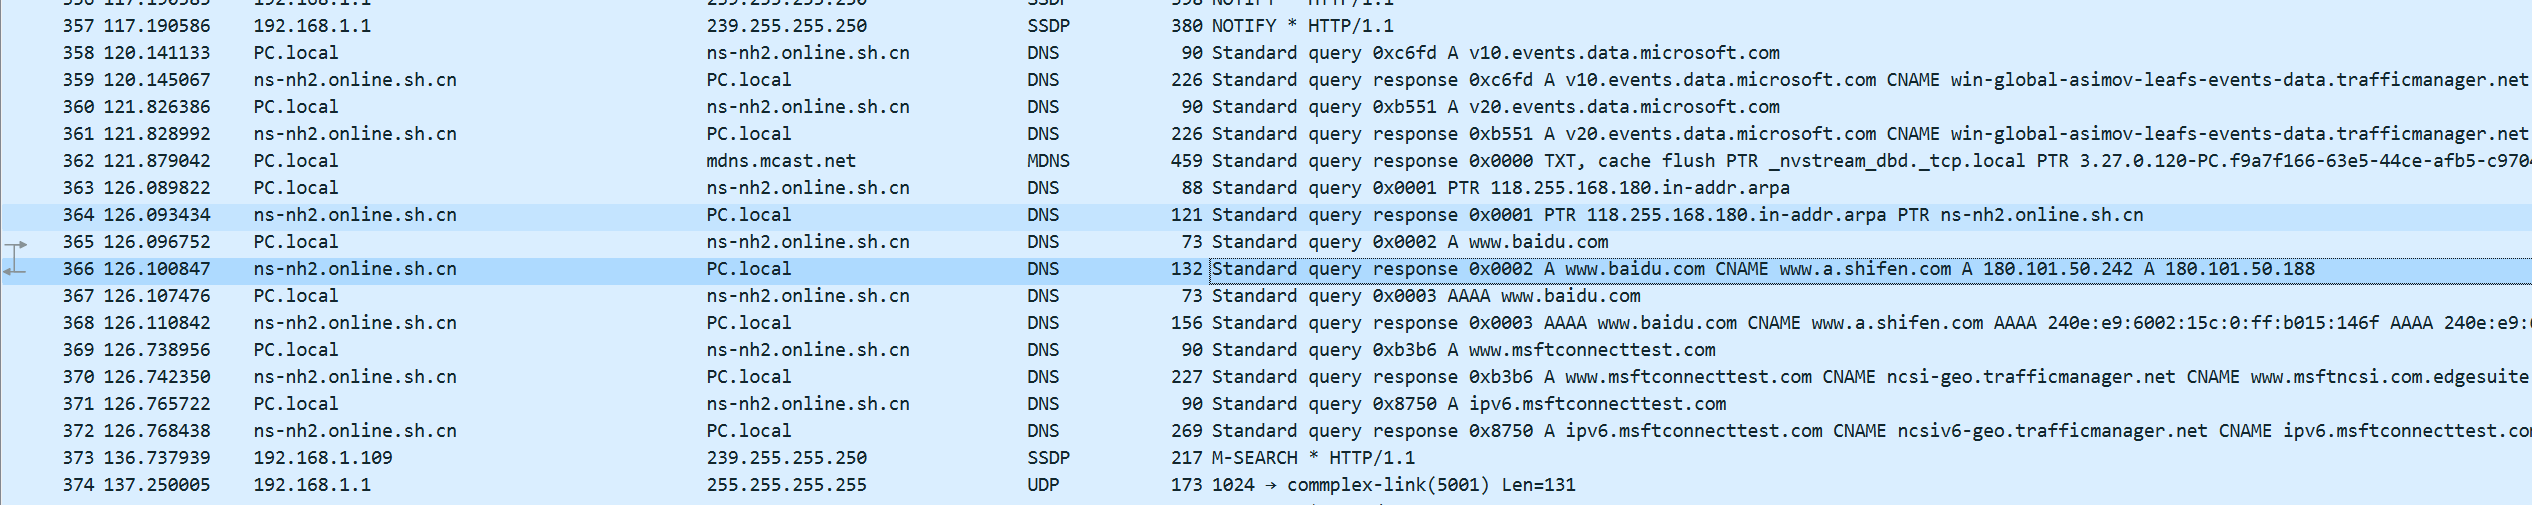
\includegraphics[width=0.8\textwidth]{img/3.png}
  \caption{捕获结果}
\end{figure}

\subsection{分析 \texttt{UDP} 包}

选择一个数据帧,分析其\texttt{UDP}包头字段。

\begin{figure}[H]
  \centering
  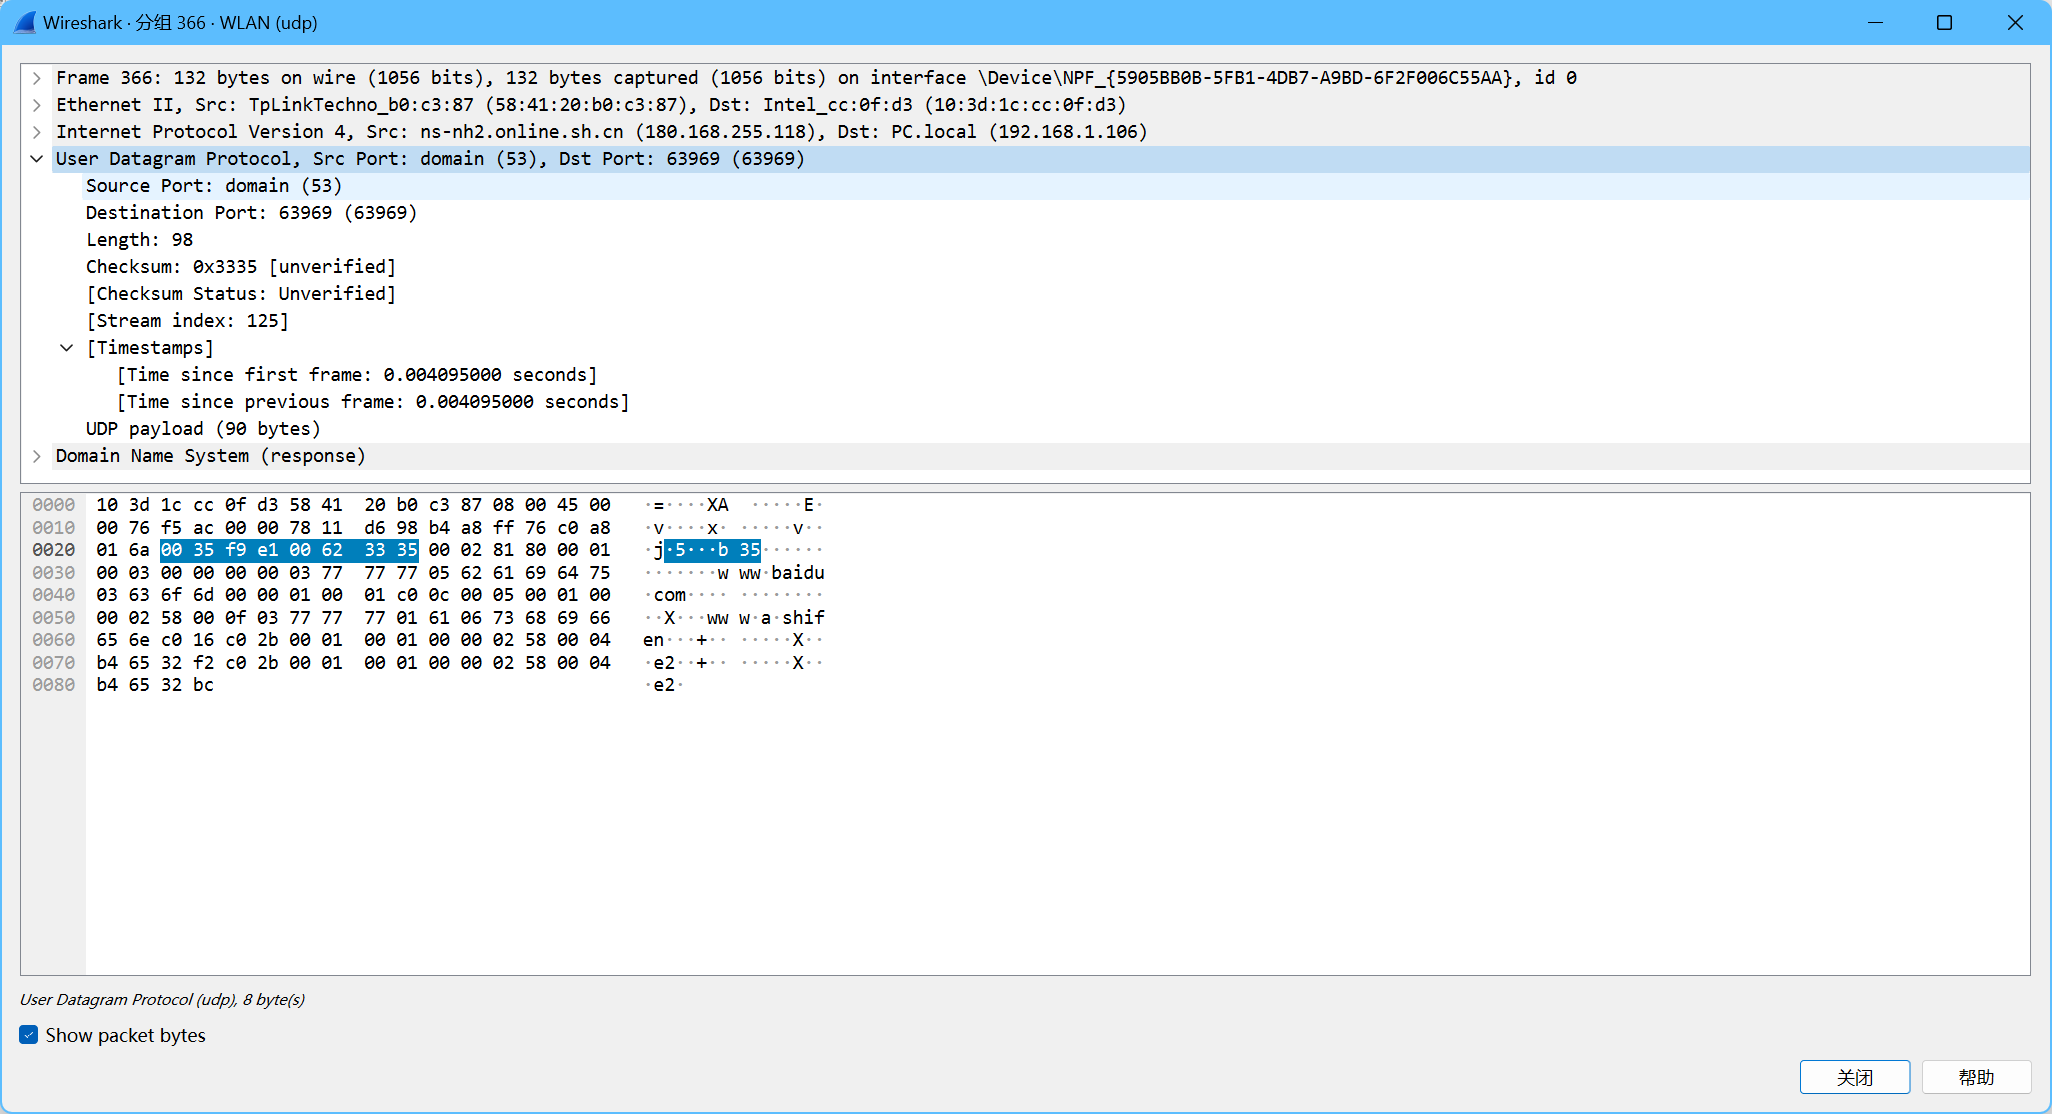
\includegraphics[width=0.75\textwidth]{img/4.png}
  \caption{\texttt{UDP}包}
\end{figure}

可以画出\texttt{UDP}包的结构如下:

% 八列的表格
\begin{table}[H]
  \centering
  \begin{tabularx}{0.8\textwidth}{|*{8}{X|}}
    \hline
    \multicolumn{2}{|X|}{源端口}      & \multicolumn{2}{|X|}{目的端口}         & \multicolumn{2}{|X|}{长度}    & \multicolumn{2}{|X|}{校验和}   \\
    \multicolumn{2}{|X|}{Source Port} & \multicolumn{2}{|X|}{Destination Port} & \multicolumn{2}{|X|}{Length}  & \multicolumn{2}{|X|}{Checksum} \\
    \multicolumn{2}{|X|}{2 bytes}     & \multicolumn{2}{|X|}{2 bytes}          & \multicolumn{2}{|X|}{2 bytes} & \multicolumn{2}{|X|}{2 bytes}  \\
    \hline
    \multicolumn{8}{|X|}{载荷}                                                                                                                  \\
    \multicolumn{8}{|X|}{Payload}                                                                                                               \\
    \multicolumn{8}{|X|}{n bytes}                                                                                                               \\
    \hline
  \end{tabularx}
  \caption{\texttt{UDP}包结构}
\end{table}

\begin{enumerate}[label={\arabic*})]
  \item \texttt{UDP}数据报头中的\texttt{Length}字段指的是\texttt{UDP}有效载荷?还是\texttt{UDP}有效载荷加上\texttt{UDP}头的总长度?还是\texttt{UDP}有效载荷和\texttt{UDP}头以及低层协议的头部三者总长度?

        在上面的 \texttt{UDP} 包中,\texttt{Payload} 长度为 90 字节,\texttt{UDP} 头长度为 8 字节,而 \texttt{Length} 字段的值为 98。

        因此可以得出 \texttt{UDP} 数据报头中的 \texttt{Length} 字段指的是 \texttt{UDP} 有效载荷加上 \texttt{UDP} 头的总长度。

  \item \texttt{UDP}头中的校验和的长度是多少位?

        \texttt{UDP}头中的校验和的长度是16位。

  \item 整个\texttt{UDP}头的长度是多少字节?

        整个\texttt{UDP}头的长度是8字节。

\end{enumerate}

启动命令行,输入\texttt{ipconfig}获得计算机的\texttt{IP}地址,与数据包中的\texttt{Source Port}比较。

\begin{figure}[H]
  \centering
  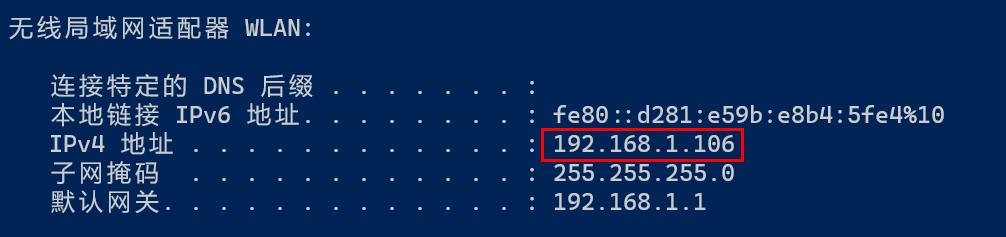
\includegraphics[width=0.8\textwidth]{img/5.png}
  \caption{\texttt{IP}地址}
\end{figure}

可以看到,\texttt{IP}地址为 \texttt{192.168.1.106},而数据包中的 \texttt{Source Port} 为 \texttt{63969},两者不同。

\begin{figure}[H]
  \centering
  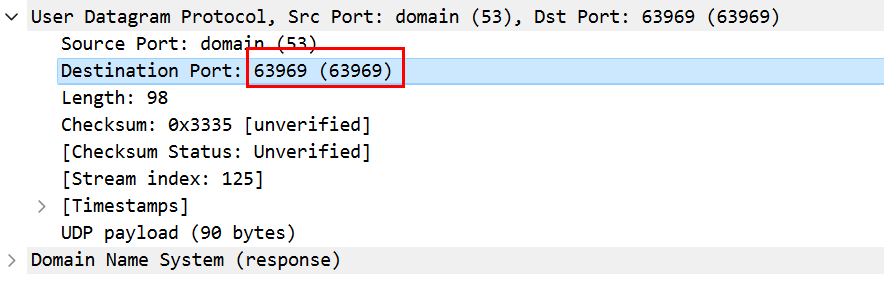
\includegraphics[width=0.8\textwidth]{img/6.png}
  \caption{\texttt{Source Port}}
\end{figure}

\begin{enumerate}[label={\arabic*})]
  \item 在\texttt{IP}协议中哪个字段指明交给上一层的\texttt{UDP}传输进程?该字段值是多少?

        在\texttt{IP}协议中,\texttt{Protocol}字段指明交给上一层的\texttt{UDP}传输进程,该字段值为 \texttt{17}。

        \begin{figure}[H]
          \centering
          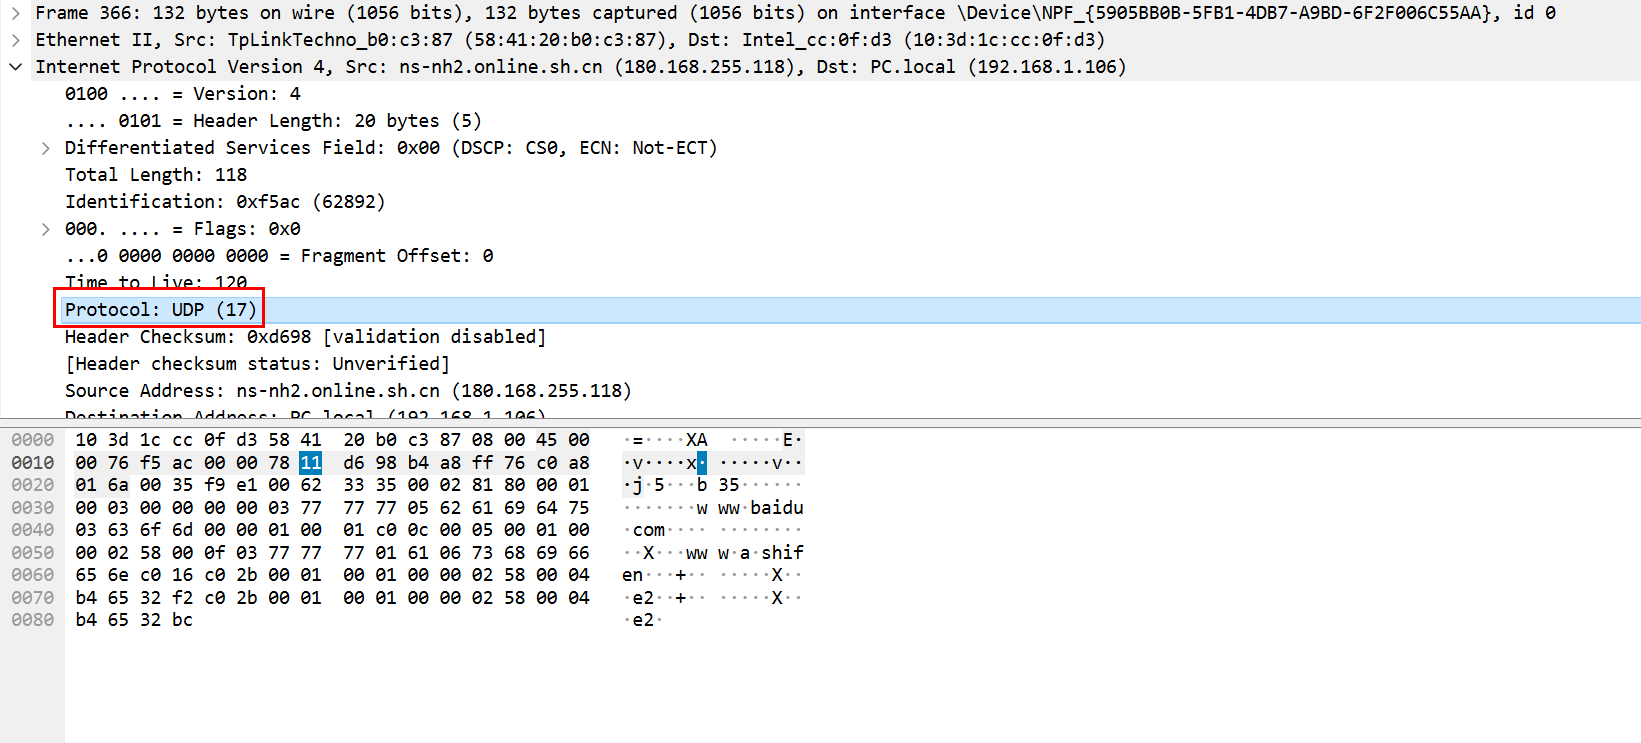
\includegraphics[width=0.8\textwidth]{img/7.png}
          \caption{\texttt{Protocol}字段}
        \end{figure}

  \item 查看源\texttt{IP}地址与目的\texttt{IP}地址都不是你的计算机的\texttt{IP}地址的数据包,并给出这些数据包的目的\texttt{IP}地址。

        \begin{figure}[H]
          \centering
          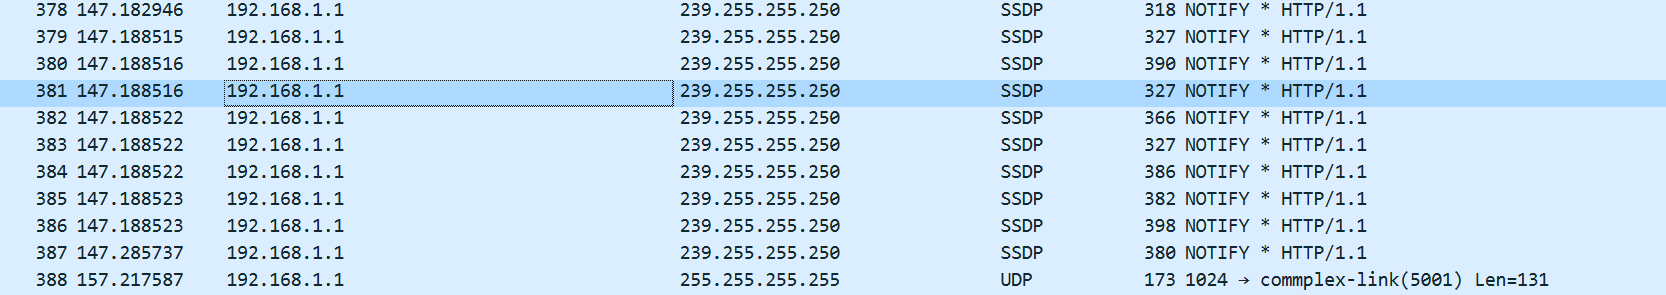
\includegraphics[width=0.8\textwidth]{img/8.png}
          \caption{数据包}
        \end{figure}

        可以看到,这些数据包的目的\texttt{IP}地址为 \texttt{239.255.255.250}

  \item 一般\texttt{UDP}消息的长度是多少?

        由于\texttt{UDP}报头中\texttt{Length}长度为 \texttt{2 Bytes},即最大长度可以达到$2^{16}-1$即65535字节。但由于以太网一帧的最大载荷为1500字节,\texttt{IP}报头为20字节,也就是说\texttt{UDP}消息总长度不能超过1480字节。

\end{enumerate}

\subsection{问题讨论}

\begin{enumerate}[noitemsep]
  \item 了解基于\texttt{UDP}的应用程序的流量,查看数据包大小和丢失率。

        QQ 采用的 \texttt{OICQ} 协议是基于 \texttt{UDP} 的,因此可以捕获 QQ 的数据包来分析。

        \begin{figure}[H]
          \centering
          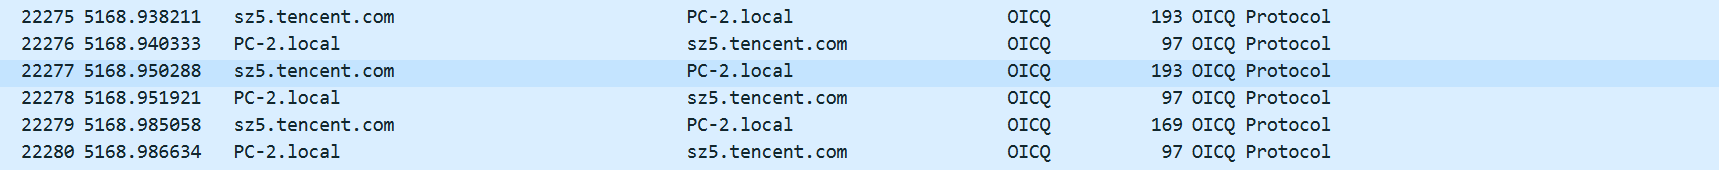
\includegraphics[width=0.8\textwidth]{img/9.png}
          \caption{捕获到的 \texttt{OICQ} 数据包}
        \end{figure}

        选择一个 \texttt{OICQ} 数据包。

        \begin{figure}[H]
          \centering
          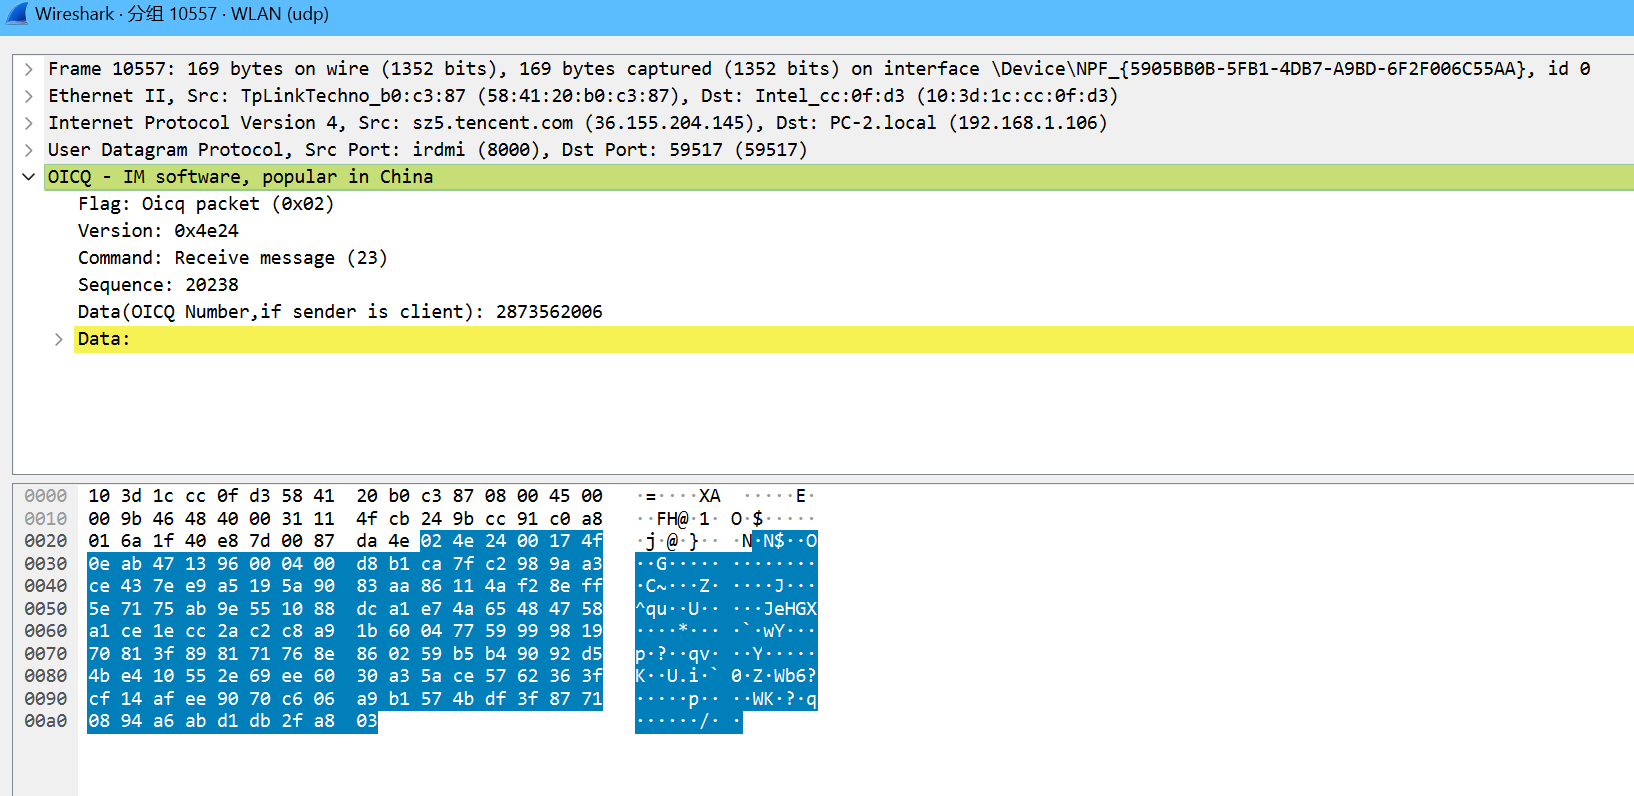
\includegraphics[width=0.8\textwidth]{img/10.png}
          \caption{\texttt{OICQ} 数据包}
        \end{figure}

        可以看到,\texttt{OICQ} 数据包的长度为 647 字节。

  \item 探索流和实时应用程序,查看哪些使用\texttt{UDP}以及哪些使用\texttt{TCP}进行传输。
  
  由于文件传输需要保证数据的完整性,因此文件传输一般使用 TCP 协议,而流媒体传输、实时通讯则可以使用 UDP 协议,因为即使丢包也不会产生太大影响,时效性更重要。

\end{enumerate}

\section{实验结果总结}

通过本次实验,我学会了通过 \texttt{Wireshark} 获取\texttt{UDP}消息,掌握了\texttt{UDP}数据包结构,掌握了\texttt{UDP}数据包各字段的含义,了解了\texttt{UDP}协议适用领域。

\section{附录}

无

\end{document}